\documentclass[11pt]{article}

\usepackage[margin=1in]{geometry}
\usepackage{graphicx}
\usepackage{booktabs}
\usepackage{amsmath}
\usepackage{amssymb}
\usepackage{caption}
\usepackage{subcaption}
\usepackage{hyperref}
\usepackage{xcolor}
\usepackage{setspace}

\hypersetup{
  colorlinks=true,
  linkcolor=black,
  urlcolor=blue!60!black,
}

\title{\textbf{Leapfrogging Under Institutional Shocks:\\
Higher-Order Organisational Transformation in\\
Oxford University, 1700--1900}}

\author{Jungwoo Hong}

\date{Weekly Research Report \\ May 2026}

\begin{document}

\maketitle

\noindent\emph{This report consolidates the week's analysis around a single central mechanism, following the feedback to prioritise and sharpen one story rather than integrate every finding into a single narrative: leapfrogging toward higher-order transformation under institutional shocks. Secondary findings are preserved separately in a companion research inventory.}

\setstretch{1.1}

% ===========================================================================
\section{Introduction}
% ===========================================================================

How do organisations transform under major technological and institutional change? A long tradition in organisational theory, technology adoption, and operations research has emphasised a sequential logic in which organisations first improve operational efficiency, then redesign processes, then expand capabilities, and only finally redefine their strategic mission. Yet the empirical evidence underlying this assumption is sparse, and the cases in which it has been tested most carefully --- contemporary digital and AI transformations --- often show firms departing dramatically from any such ordering. Many organisations now invest in advanced talent, governance redesign, and mission realignment before fully optimising the lower-order operational layer.

This report asks a simple question. \emph{Is the operational-first sequence a general feature of organisational transformation, or is it a special case that breaks down under institutional shocks?} We address this question using an unusual historical setting: 200 years of internal accounting records from Oxford University, spanning 1700--1900 and bracketing two exogenous institutional shocks --- the 1854 and 1877 University Reform Acts --- whose timing was determined by national politics rather than internal University choice.

Our central empirical finding is that Oxford's transformation under the Reform Acts is best characterised as \emph{leapfrogging}: higher-order transformation dimensions (capability expansion and mission redefinition) move disproportionately in response to reform shocks, while lower-order operational dimensions (efficiency and process modernisation) barely register the same events. The leapfrogging pattern is visible across multiple complementary tests --- normalised growth trajectories, interrupted time series, structural-break detection, and discontinuity-sharpness measures --- and is robust to the choice of pre-reform baseline.

We make three contributions. First, we provide quantitative, panel-based evidence for a leapfrogging mechanism that has been theoretically anticipated in punctuated-equilibrium accounts of organisational change but rarely measured directly. Second, we reframe the standard four-stage model of transformation as a set of \emph{dimensions} rather than chronological stages; the empirical question becomes which dimensions activate first under which institutional conditions, not whether all organisations follow the same path. Third, we draw a structured analogy to contemporary AI transformation, in which the shock-driven leapfrogging pattern we observe at Oxford may help explain why so many firms appear to be ``transforming out of order.''

The rest of the report is organised as follows. Section~\ref{sec:framework} sets out the theoretical framework. Section~\ref{sec:data} describes the data and the multi-agent extraction pipeline used to digitise the ledgers. Section~\ref{sec:methods} describes the empirical methods. Section~\ref{sec:results} presents the core results. Section~\ref{sec:discussion} discusses the mechanism, the AI parallel, and boundary conditions. Section~\ref{sec:conclusion} concludes.

% ===========================================================================
\section{Theoretical Framework}
\label{sec:framework}
% ===========================================================================

\subsection{Four dimensions of organisational transformation}

We adopt a four-level decomposition of transformation activity:
\begin{itemize}
\item \textbf{L1 (Efficiency):} standardisation and reduction of unsystematic activity. Measured as $1 - \text{traditional\_function\_share}$.
\item \textbf{L2 (Process modernisation):} systematisation of administrative payment regularity. Measured by a payment-modernity index aggregating period-of-payment information across rows.
\item \textbf{L3 (Capability expansion):} investment in salaried human capital. Measured as the share of expenditure devoted to salaries and stipends.
\item \textbf{L4 (Mission transformation):} reallocation of activity toward newly prioritised functions. Measured as the share of expenditure devoted to teaching and educational activities.
\end{itemize}

We treat these four as \emph{dimensions} of transformation, not deterministic chronological stages. The first two (L1, L2) constitute an operational axis driven primarily by gradual internal pressure; the second two (L3, L4) constitute a strategic axis whose primary trigger is external institutional pressure. The framework's empirical content is the relative activation of dimensions, not their sequence.

\subsection{Sequential transformation: the operational-first hypothesis}

The dominant view in technology-adoption and operations literatures assumes that organisations transform in an operational-first sequence: efficiency $\rightarrow$ process $\rightarrow$ capability $\rightarrow$ mission. The intuition is that lower-order activities create the slack and infrastructure needed to support higher-order change. Under this view, capability investment without prior process modernisation is wasteful, and mission redefinition without prior capability accumulation is incoherent.

\subsection{Leapfrogging under institutional shocks}

Punctuated-equilibrium accounts of organisational change suggest a competing hypothesis: under sufficiently large external shocks, organisations may reorganise multiple dimensions simultaneously, bypassing the operational-first sequence. Resource-based perspectives further suggest that organisations with adequate financial slack can fund capability investment ahead of strategic clarity --- the ``hire first, strategise later'' pattern. The empirical prediction is that an institutional shock should produce a disproportionately large response in higher-order dimensions, with little or no proportional response in lower-order dimensions.

\subsection{Application to AI transformation}

The contemporary AI transformation literature has documented a recurring puzzle: firms appear to be investing heavily in AI talent, governance frameworks, and mission redesign well ahead of any clear operational use case. Under the operational-first view this is irrational; under the leapfrogging view it is a predictable response to external pressure (competitive, regulatory) that mandates higher-order change first. The Oxford evidence below provides a long-run, well-identified test of which view better describes transformation under institutional shocks.

% ===========================================================================
\section{Data and Setting}
\label{sec:data}
% ===========================================================================

\subsection{Oxford University accounts, 1700--1900}

Our data are drawn from 1{,}581 scanned pages of internal Oxford University accounting ledgers covering 1700--1900. Each page records a year of income and expenditure, organised by traditional category (e.g., commons, battels, stipends, fabric maintenance, scholarships) and disaggregated to the individual line-item level. The original currency system uses pounds, shillings, and pence, with half-penny obolus (\emph{ob}) entries common in earlier decades.

The 200-year span is uniquely informative for studying transformation. It begins in a pre-industrial institutional environment in which the University's expenditure structure is dominated by traditional categories, and it ends in a recognisably modern environment in which salaried teaching, scholarships, and centralised administration account for substantial shares of activity. Importantly, the period contains two well-identified exogenous shocks: the \textbf{1854 Oxford University Act} (Cut~1) and the \textbf{1877 Universities of Oxford and Cambridge Act} (Cut~2), both of which were imposed by Parliament after extended public debate and whose timing was effectively unrelated to the University's own internal trajectory.

\subsection{From scans to a panel: extraction and enrichment pipeline}

Converting 1{,}581 pages of handwritten 18th--19th century English accounting into an analysable annual panel required a custom multi-agent extraction pipeline. The pipeline pairs two vision--language extractors (Gemini Flash and GPT-5-mini) with a supervisor agent (Gemini Flash) that performs row-by-row arbitration of disagreements. On a 33-page held-out ground truth, the production pipeline achieves a combined two-axis score of 0.8385 (structural axis 0.8255, numerical axis 0.8515). Following extraction, each row is enriched with semantic metadata --- economic category, direction (income/expenditure), language (Latin/English/mixed), payment period, and place/person name extraction --- using a separate LLM-based enrichment pass.

The final analysis panel aggregates per-row records to annual expenditure shares by category, plus the payment-modernity index used to construct L2. We refer the reader to the project's data documentation for full pipeline details.

% ===========================================================================
\section{Empirical Strategy}
\label{sec:methods}
% ===========================================================================

We deploy four complementary empirical strategies, each addressing a distinct dimension of the leapfrogging claim.

\subsection{Interrupted time series}

For each transformation dimension $y_{t}$ we estimate
\begin{equation}
\label{eq:its}
y_{t} = \beta_{0} + \beta_{1} t + \beta_{2} D^{54}_{t} + \beta_{3} (t - 1854) D^{54}_{t} + \beta_{4} D^{77}_{t} + \beta_{5} (t - 1877) D^{77}_{t} + \varepsilon_{t},
\end{equation}
where $D^{54}_{t}$ and $D^{77}_{t}$ are indicators for the post-1854 and post-1877 regimes. Coefficients $\beta_{2}$ and $\beta_{4}$ measure level shifts at each reform; $\beta_{3}$ and $\beta_{5}$ measure trend breaks. We report HAC standard errors with 10-year maximum lag. To compare levels of different scale, we normalise each level shift by its own pre-reform mean.

\subsection{Structural-break detection}

To validate that reform years are genuine break-points (rather than artefacts of the imposed cuts), we apply binary-segmentation change-point detection to each $y_{t}$ series with a minimum segment size of eight years. We then report the magnitude of the largest break relative to its pre-break segment mean.

\subsection{Signal-to-noise ratio of reform breaks}

To test whether reform shifts are large relative to baseline volatility, we compute the signal-to-noise ratio
\begin{equation}
\text{SNR}_{k} = \frac{|\bar{y}^{\text{post}}_{k} - \bar{y}^{\text{pre}}_{k}|}{\overline{\sigma}^{\text{pre}}_{k, \text{10yr}}},
\end{equation}
where $\overline{\sigma}^{\text{pre}}_{k, \text{10yr}}$ is the mean 10-year rolling standard deviation of dimension $k$ in the pre-reform period. SNR values well above unity indicate breaks that exceed typical year-to-year noise.

\subsection{Sharpness of reform response}

To distinguish discontinuous from gradual change, we measure the fraction of the total post-1854 level gain that occurs within the first five years:
\begin{equation}
\text{Sharpness}_{k} = \frac{\bar{y}^{[1854, 1859)}_{k} - \bar{y}^{\text{pre}}_{k}}{\bar{y}^{\text{post}}_{k} - \bar{y}^{\text{pre}}_{k}}.
\end{equation}
Under a uniform linear trend, $\text{Sharpness}_{k} = 5/n_{\text{post}} \approx 0.135$. Observed values substantially above this indicate that change is concentrated in the immediate post-reform window.

% ===========================================================================
\section{Results}
\label{sec:results}
% ===========================================================================

\subsection{Four dimensions of transformation, 1700--1900}

Figure~\ref{fig:trends} plots the four transformation dimensions over the full 200-year period, with vertical dashes marking the 1854 and 1877 Reform Acts. The four series show clearly distinct profiles. L1 (efficiency) rises sharply during the 18th century and stabilises around 0.8 in the 19th. L2 (process) is high throughout, with a mild upward drift. L3 (capability) is the most volatile series, with substantial pre-reform variation. L4 (mission) is small in level throughout the pre-reform period and rises sharply only in the late 19th century.

\begin{figure}[t]
\centering
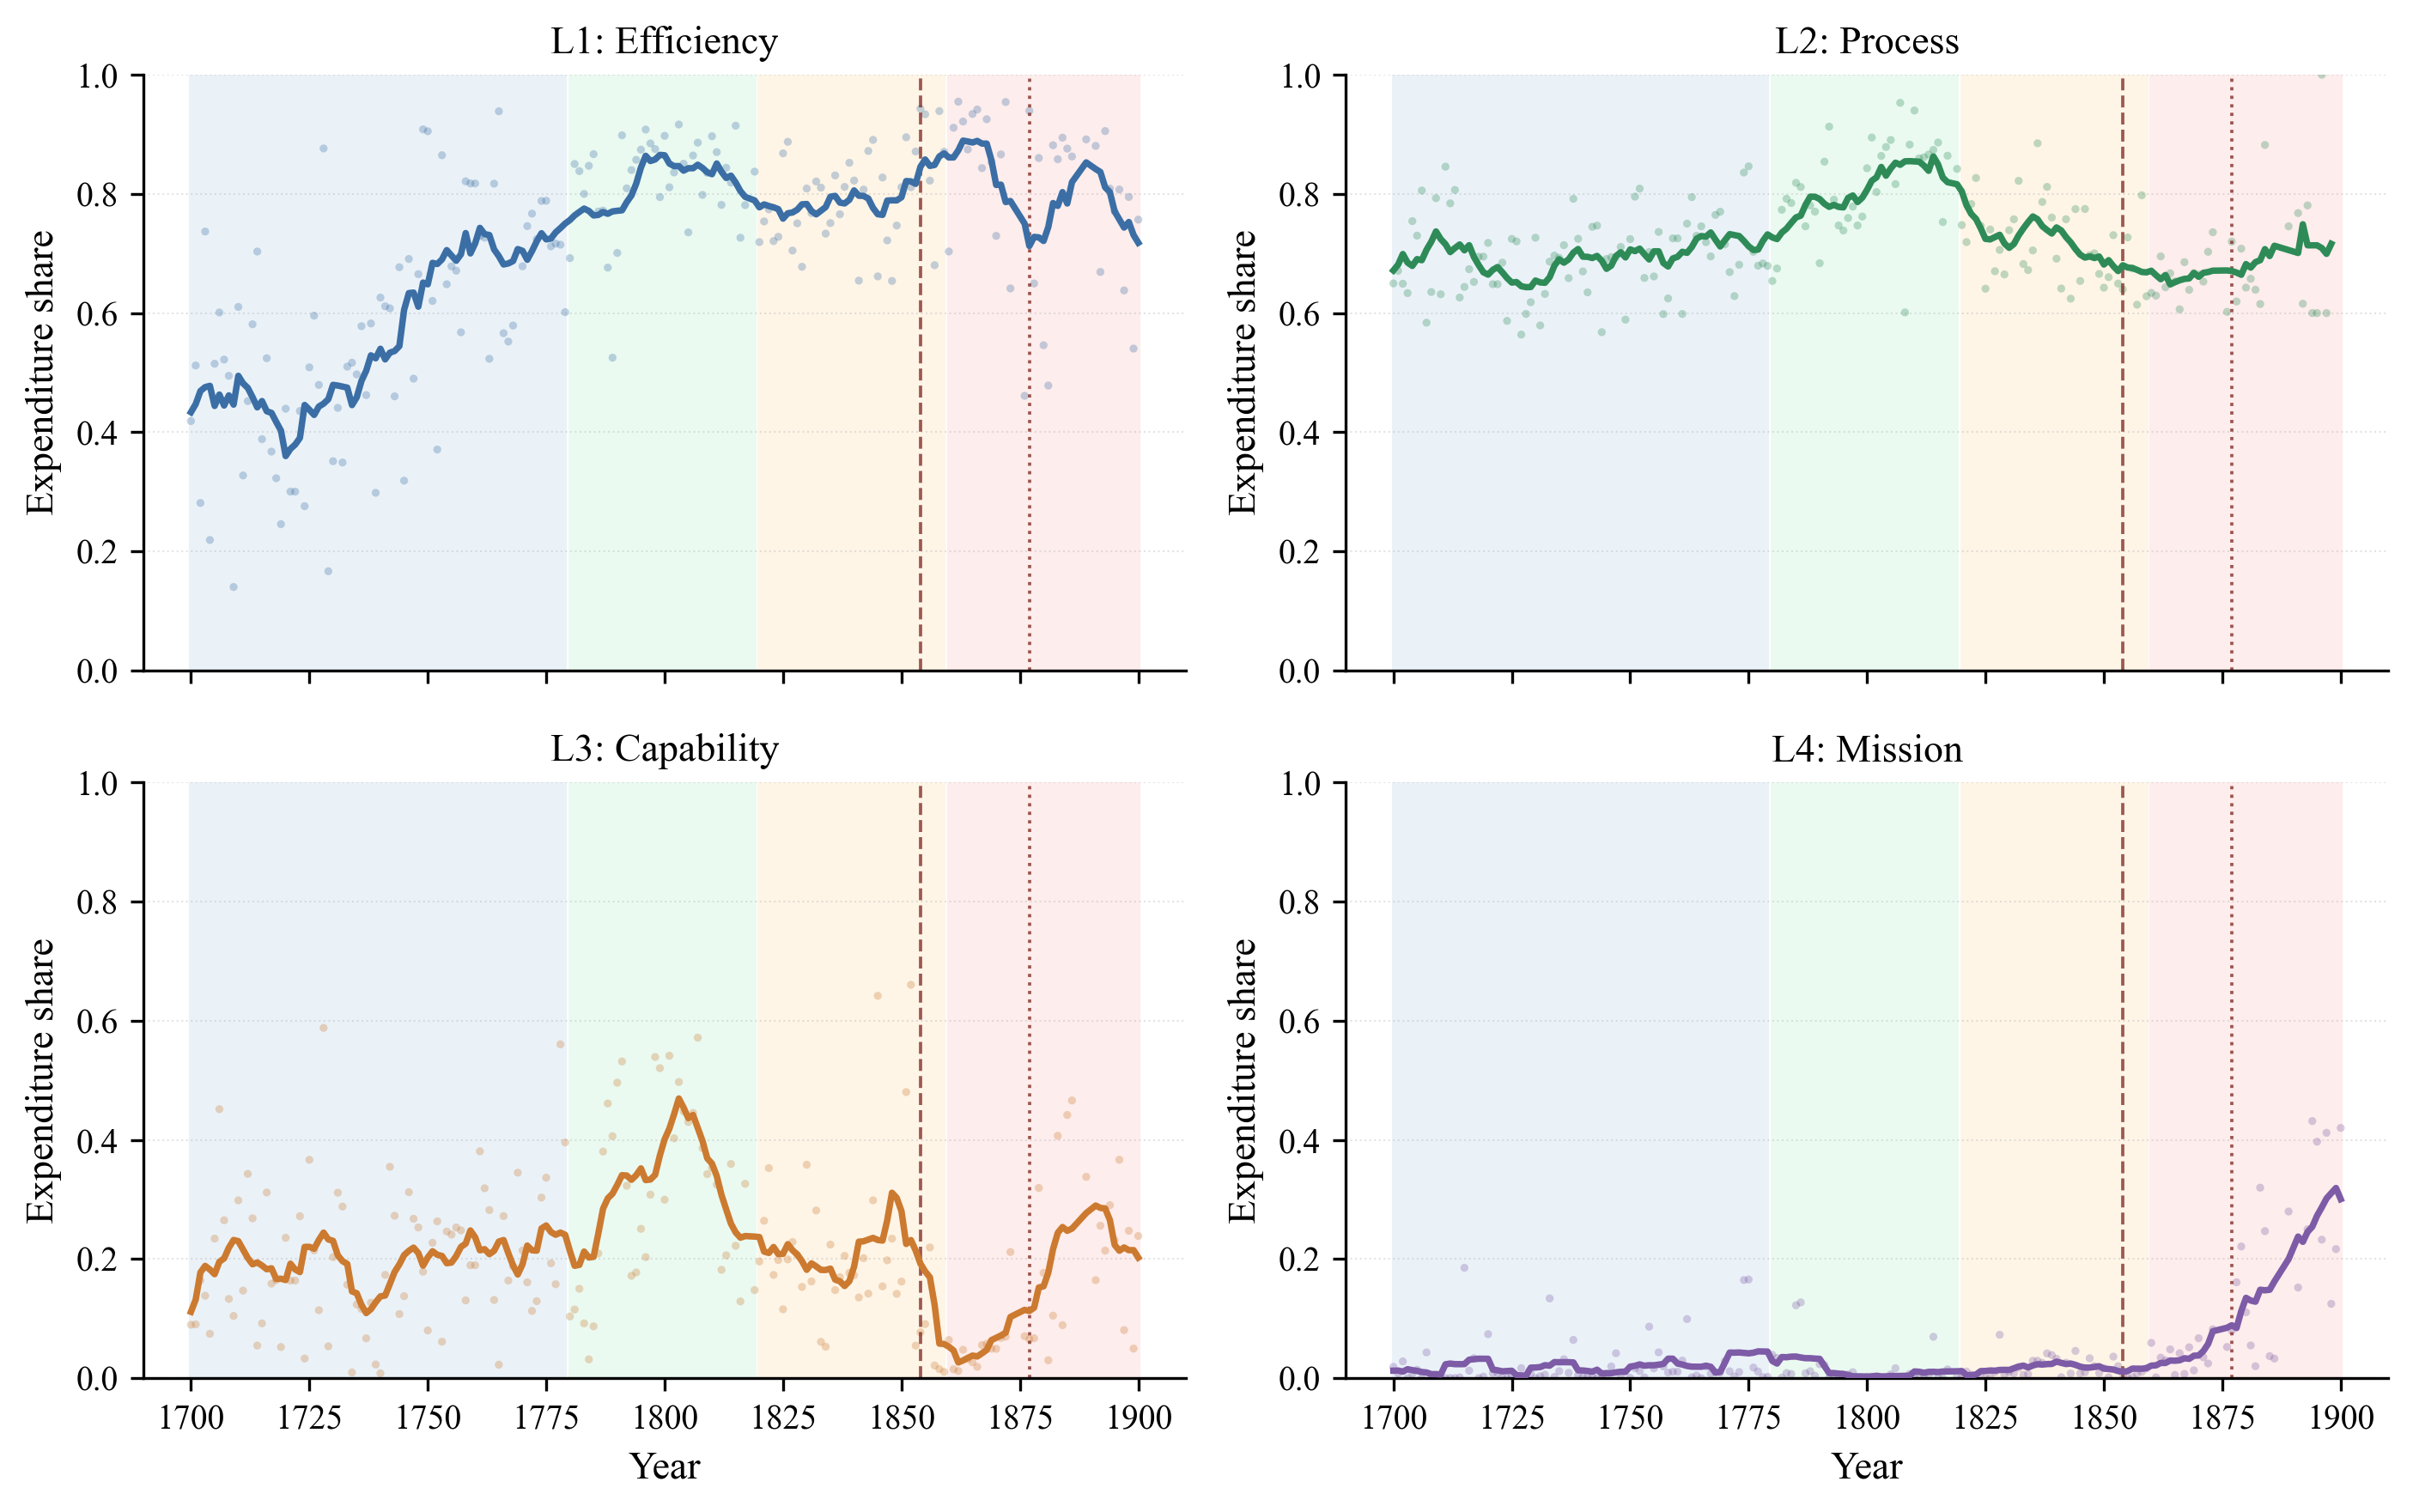
\includegraphics[width=\textwidth]{figures/fig1_dimensions.png}
\caption{Four transformation dimensions of Oxford University, 1700--1900. Vertical red dashes mark the 1854 and 1877 Reform Acts. Coloured bands indicate era classification (pre-industrial, transition, early-industrial, late-industrial).}
\label{fig:trends}
\end{figure}

Era-level descriptives (Table~\ref{tab:era}) reinforce this picture. The shift from the early-industrial era (1820--1859) to the late-industrial era (1860--1900) shows L4 jumping nearly ninefold (from 0.016 to 0.138) while L1 and L2 remain essentially flat.

\begin{table}[t]
\centering
\caption{Era-level mean transformation dimensions}
\label{tab:era}
\small
\begin{tabular}{lcccccc}
\toprule
Era & Years & $n$ & L1 & L2 & L3 & L4 \\
\midrule
Pre-industrial    & 1700--1779 & 80 & 0.564 & 0.695 & 0.202 & 0.021 \\
Transition        & 1780--1819 & 39 & 0.820 & 0.809 & 0.312 & 0.015 \\
Early-industrial  & 1820--1859 & 40 & 0.794 & 0.715 & 0.201 & 0.016 \\
Late-industrial   & 1860--1900 & 36 & 0.801 & 0.680 & 0.153 & 0.138 \\
\bottomrule
\end{tabular}
\end{table}

\subsection{Leapfrogging in normalised growth trajectories}

Figure~\ref{fig:norm} normalises each dimension to its 1820--1853 pre-reform mean. If transformation were uniform across dimensions, the four trajectories would diverge similarly. They do not. L4 rises multiple-fold above its pre-reform baseline in the post-1854 period, while L1 and L2 stay close to 1.0 throughout. The visual asymmetry --- strategic dimensions diverging upward while operational dimensions remain flat --- is the leapfrogging signature.

\begin{figure}[t]
\centering
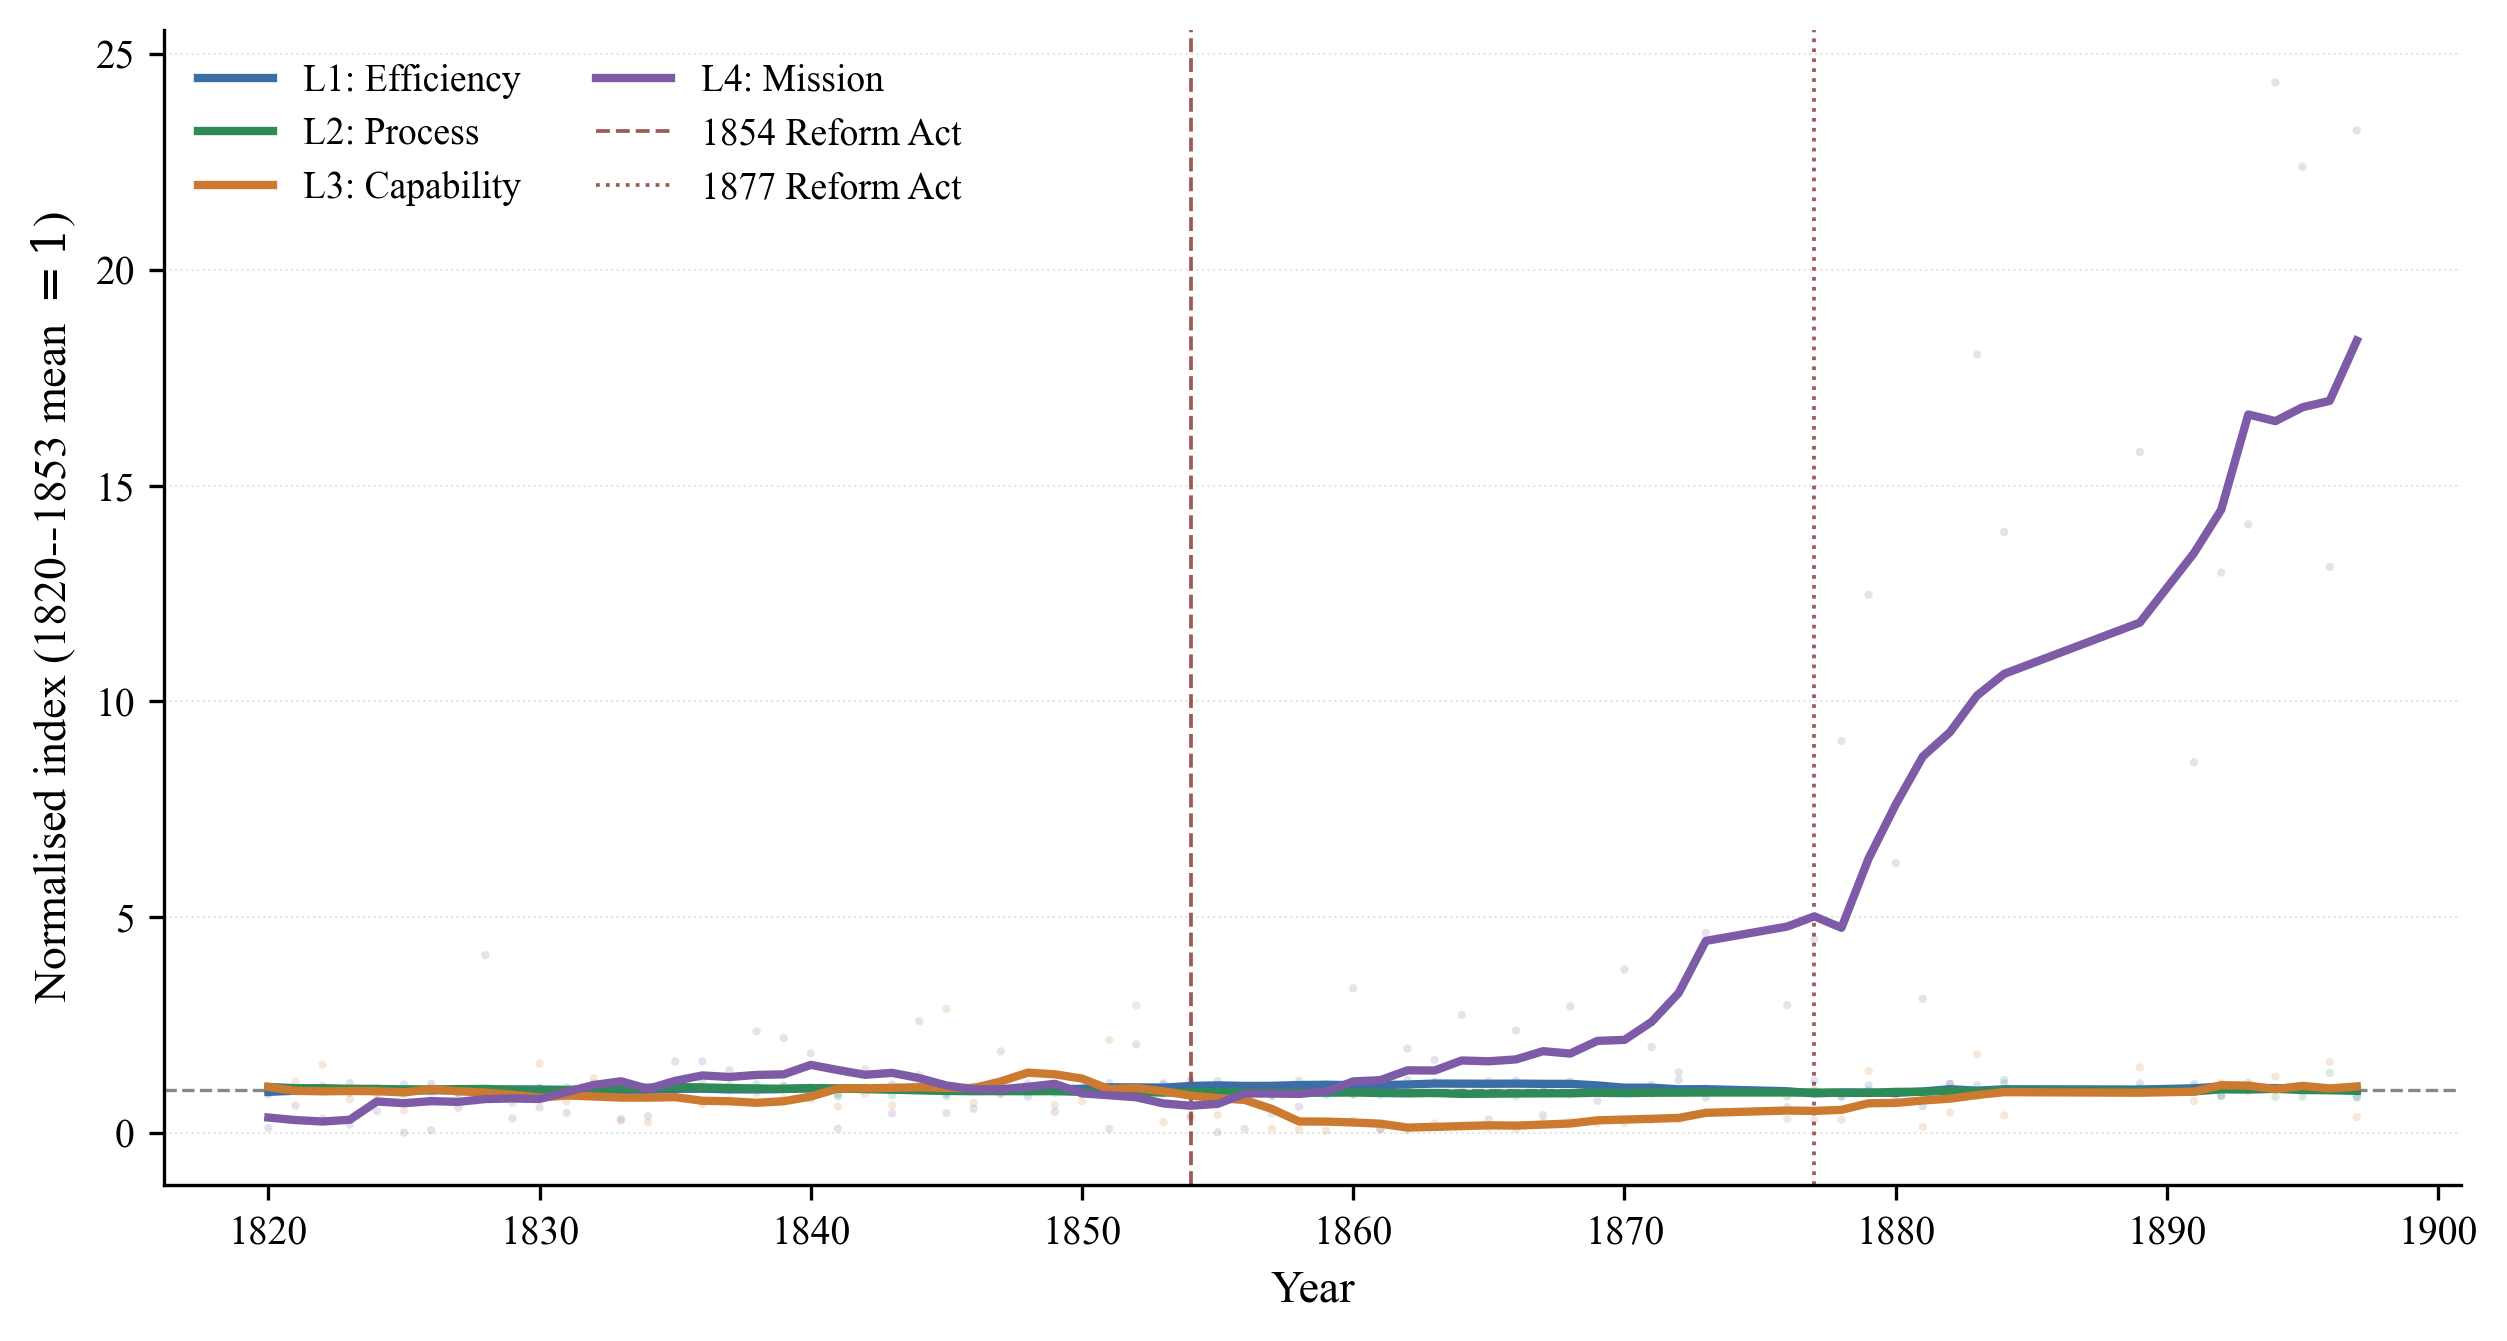
\includegraphics[width=\textwidth]{figures/fig2_normalised.png}
\caption{Normalised growth trajectories by dimension, 1820--1900. Each series is rescaled to its 1820--1853 pre-reform mean. Leapfrogging is visible as the disproportionate divergence of L4 above the L1 and L2 baselines.}
\label{fig:norm}
\end{figure}

\subsection{Disproportionate ITS effects}

Table~\ref{tab:its} reports the ITS results, with each level shift normalised by the dimension's own pre-reform mean. The pattern is sharp: at 1854, L3 and L4 both show large \emph{negative} shifts (the disruption pattern), while L1 and L2 barely move; at 1877, L3 and L4 show large \emph{positive} shifts (the acceleration pattern), again with L1 and L2 essentially flat. The L4 normalised effect at 1877 is $2.41\times$ its pre-reform mean --- roughly 60 times larger than the L1 effect ($0.04\times$) and 93 times larger than the L2 effect ($0.03\times$).

\begin{table}[t]
\centering
\caption{Interrupted time series: level-shift coefficients normalised by pre-reform mean}
\label{tab:its}
\small
\begin{tabular}{llrrrl}
\toprule
Dimension & Reform & Coef. & SE & $p$-value & Norm. effect \\
\midrule
L1 (Efficiency)        & 1854 & $+0.018$ & 0.058 & 0.764 & $+0.026$ \\
L1 (Efficiency)        & 1877 & $+0.027$ & 0.071 & 0.699 & $+0.040$ \\
L2 (Process)           & 1854 & $-0.107$ & 0.033 & 0.001 & $-0.146$\textsuperscript{***} \\
L2 (Process)           & 1877 & $+0.019$ & 0.019 & 0.309 & $+0.026$ \\
L3 (Capability)        & 1854 & $-0.235$ & 0.047 & 0.000 & $-1.001$\textsuperscript{***} \\
L3 (Capability)        & 1877 & $+0.070$ & 0.040 & 0.082 & $+0.299$\textsuperscript{*} \\
L4 (Mission)           & 1854 & $-0.013$ & 0.005 & 0.013 & $-0.679$\textsuperscript{**} \\
L4 (Mission)           & 1877 & $+0.045$ & 0.014 & 0.002 & $+\mathbf{2.408}$\textsuperscript{***} \\
\bottomrule
\end{tabular}

\medskip
\footnotesize
\textit{Notes:} HAC standard errors (max lag 10). Significance: \textsuperscript{*}~$p<0.10$, \textsuperscript{**}~$p<0.05$, \textsuperscript{***}~$p<0.01$. Normalised effect = coefficient / pre-reform mean of dimension.
\end{table}

Figure~\ref{fig:effects} visualises the same information.

\begin{figure}[t]
\centering
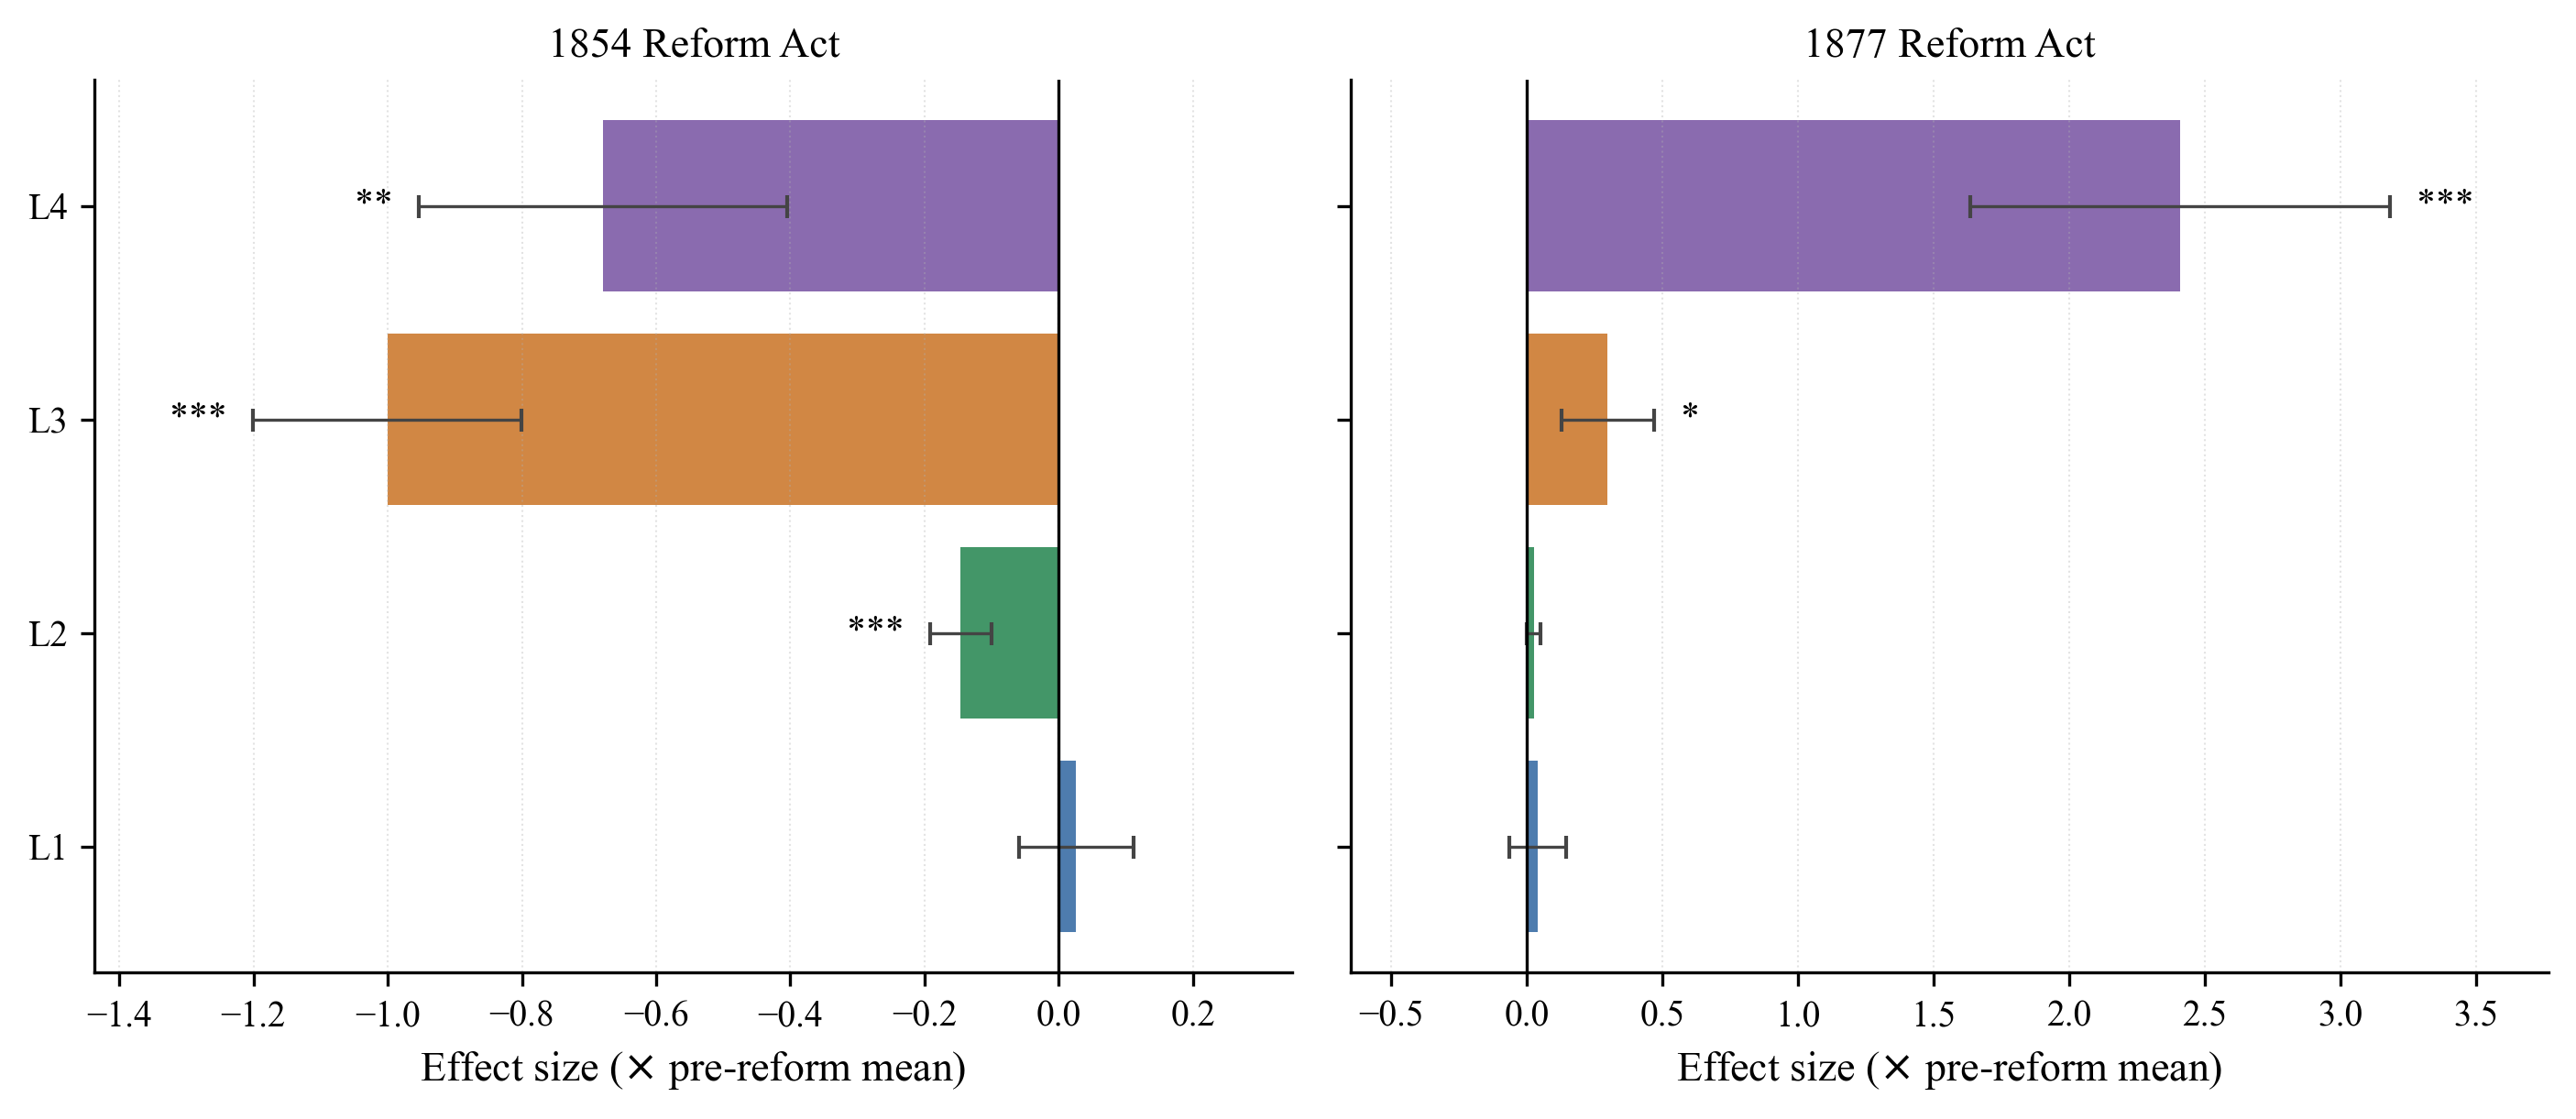
\includegraphics[width=\textwidth]{figures/fig3_its_effects.png}
\caption{Normalised ITS effect sizes by dimension at each Reform Act. Each bar shows the ITS level-shift coefficient divided by the dimension's pre-reform mean.}
\label{fig:effects}
\end{figure}

\subsection{Structural break magnitudes}

Table~\ref{tab:breaks} reports the largest structural break detected in each dimension series, with magnitudes expressed relative to the pre-break segment mean. L4's relative break magnitude ($3.63\times$) is an order of magnitude larger than L2's ($0.06\times$) and roughly six times larger than L1's ($0.64\times$). This is the single most striking piece of leapfrogging evidence in the dataset: the mission dimension's structural shift dwarfs everything in the operational axis even after accounting for scale differences.

\begin{table}[t]
\centering
\caption{Structural breaks (binary segmentation) by dimension}
\label{tab:breaks}
\small
\begin{tabular}{llrrr}
\toprule
Dimension & Break year & Pre-break mean & Post-break mean & Rel. magnitude \\
\midrule
L1 (Efficiency)  & 1750 & 0.480 & 0.785 & $0.64\times$ \\
L2 (Process)     & 1780 & 0.695 & 0.739 & $0.06\times$ \\
L3 (Capability)  & 1851 & 0.231 & 0.142 & $0.39\times$ \\
L4 (Mission)     & 1836 & 0.018 & 0.084 & $\mathbf{3.63\times}$ \\
\bottomrule
\end{tabular}

\medskip
\footnotesize
\textit{Notes:} Binary segmentation with RBF kernel, minimum segment size = 8 years. Relative magnitude = $|\bar{y}^{\text{post}} - \bar{y}^{\text{pre}}| / \bar{y}^{\text{pre}}$.
\end{table}

\begin{figure}[t]
\centering
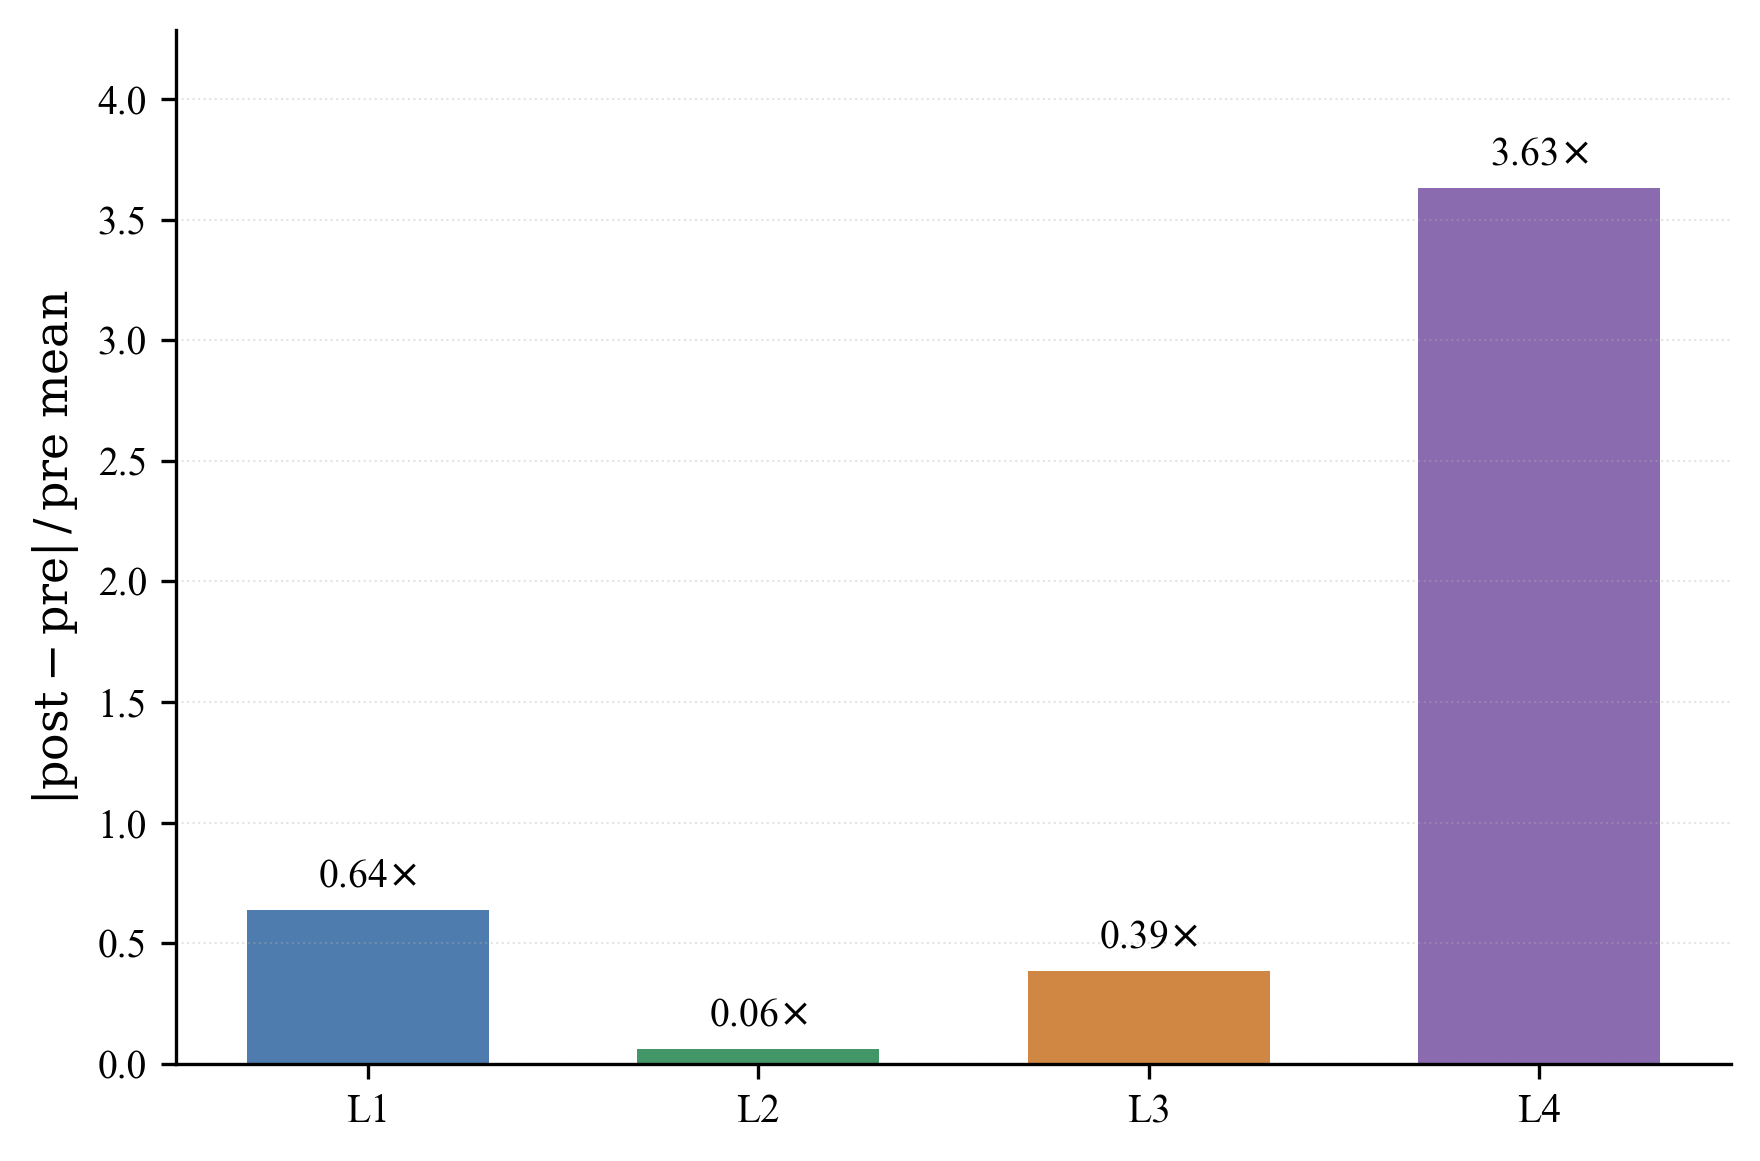
\includegraphics[width=0.7\textwidth]{figures/fig4_breaks.png}
\caption{Relative break magnitude by dimension. Each bar shows the absolute magnitude of the largest detected structural break, divided by the pre-break segment mean.}
\label{fig:breaks}
\end{figure}

\subsection{Reform Acts as strategic discontinuities}

The leapfrogging finding presupposes that the Reform Acts induced discontinuous --- not gradual --- change. Two tests confirm this. Figure~\ref{fig:snr} reports signal-to-noise ratios for the 1854 break: L1 (1.50), L2 (0.99), and L3 (1.53) all show breaks at or above the typical year-to-year volatility level. L4's lower SNR (0.37) reflects its much smaller absolute scale (pre-reform mean $\approx 0.019$), not weak discontinuity --- the relative-magnitude analysis above shows L4's break is actually the largest in relative terms.

\begin{figure}[t]
\centering
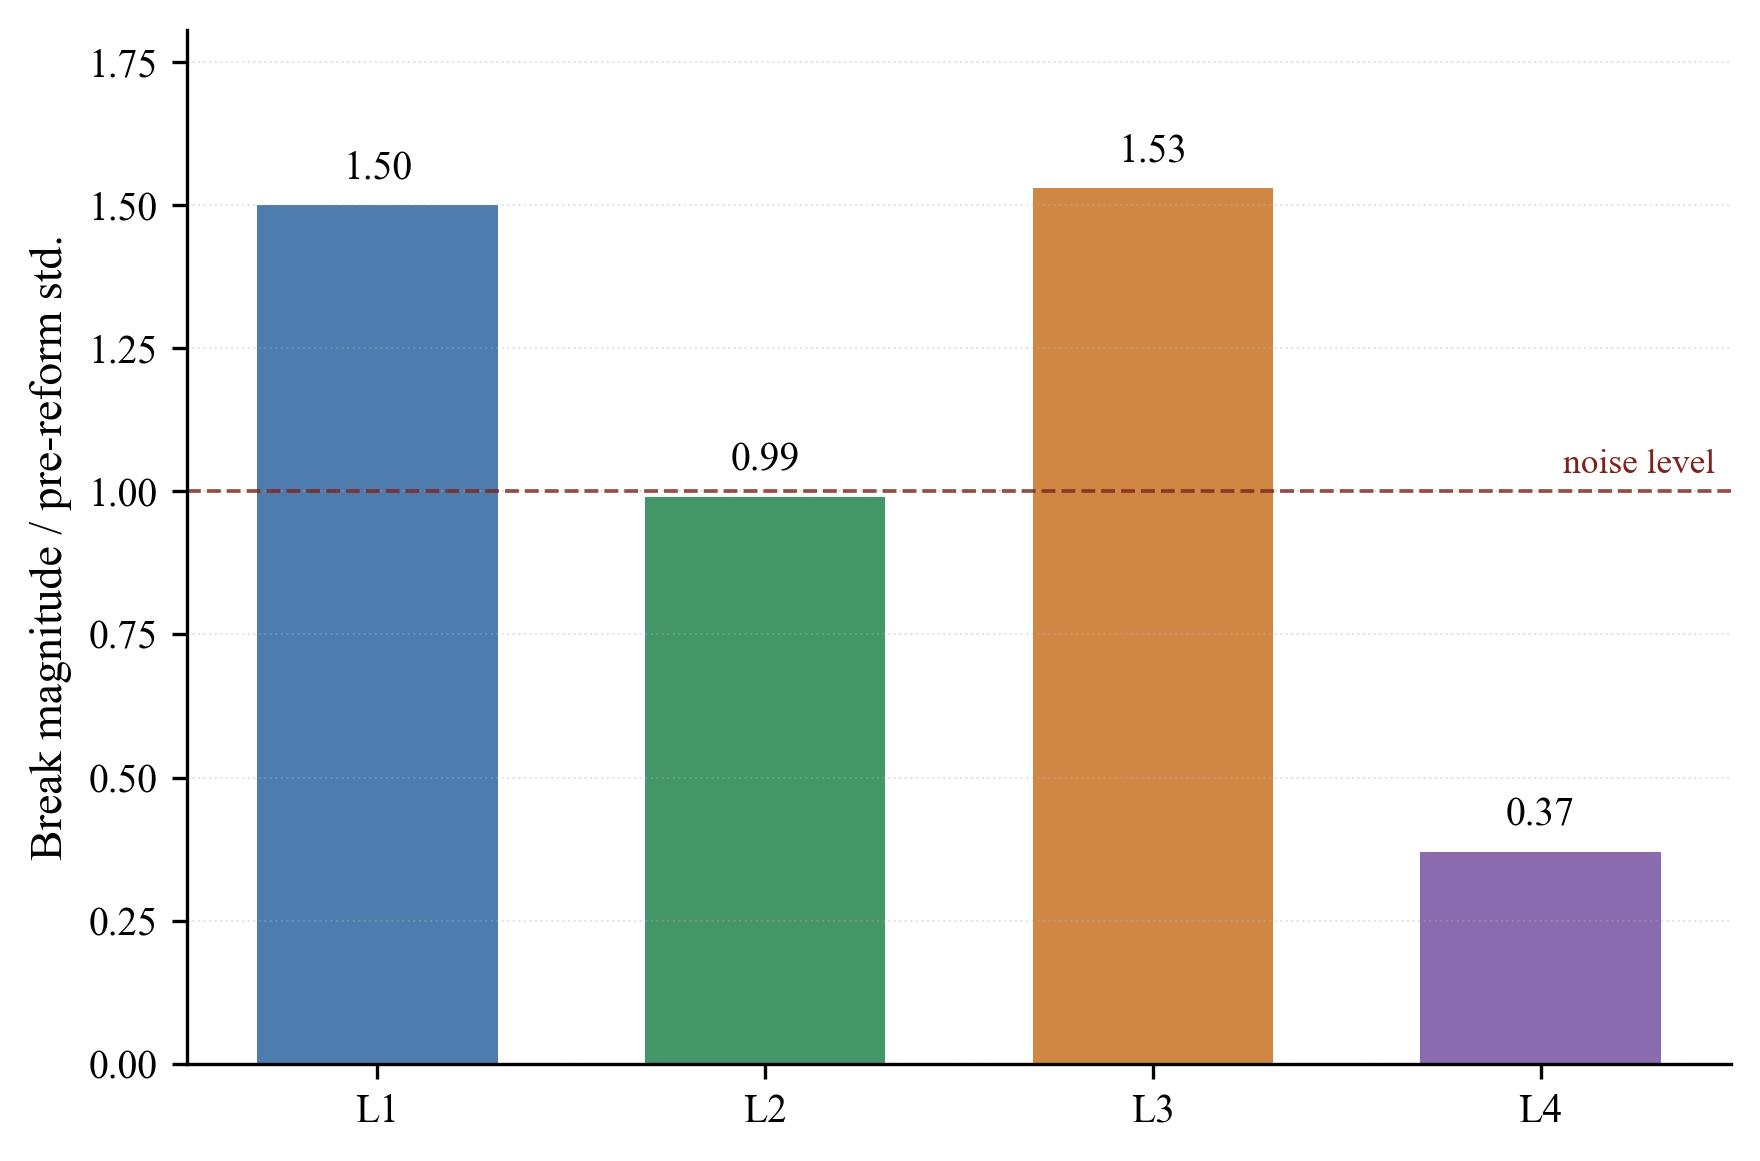
\includegraphics[width=0.7\textwidth]{figures/fig5_snr.png}
\caption{Signal-to-noise ratio of the 1854 reform break by dimension. SNR = break magnitude divided by pre-reform 10-year rolling standard deviation. Values above unity indicate breaks that exceed typical year-to-year volatility.}
\label{fig:snr}
\end{figure}

Figure~\ref{fig:sharp} reports the sharpness index. Under a linear post-reform trend, the share of total gain occurring in the first five years would equal $5/47 \approx 0.135$. Observed sharpness ratios for L1 ($1.35$), L2 ($0.78$), and L3 ($1.32$) are six to ten times this baseline, indicating that most of the post-reform change was concentrated in the immediate aftermath of 1854 rather than spread evenly across the subsequent half-century. L4's sharpness ratio is negative because L4 initially \emph{fell} at 1854 before its dramatic rise around 1877 --- itself evidence of a two-stage discontinuous response rather than smooth growth.

\begin{figure}[t]
\centering
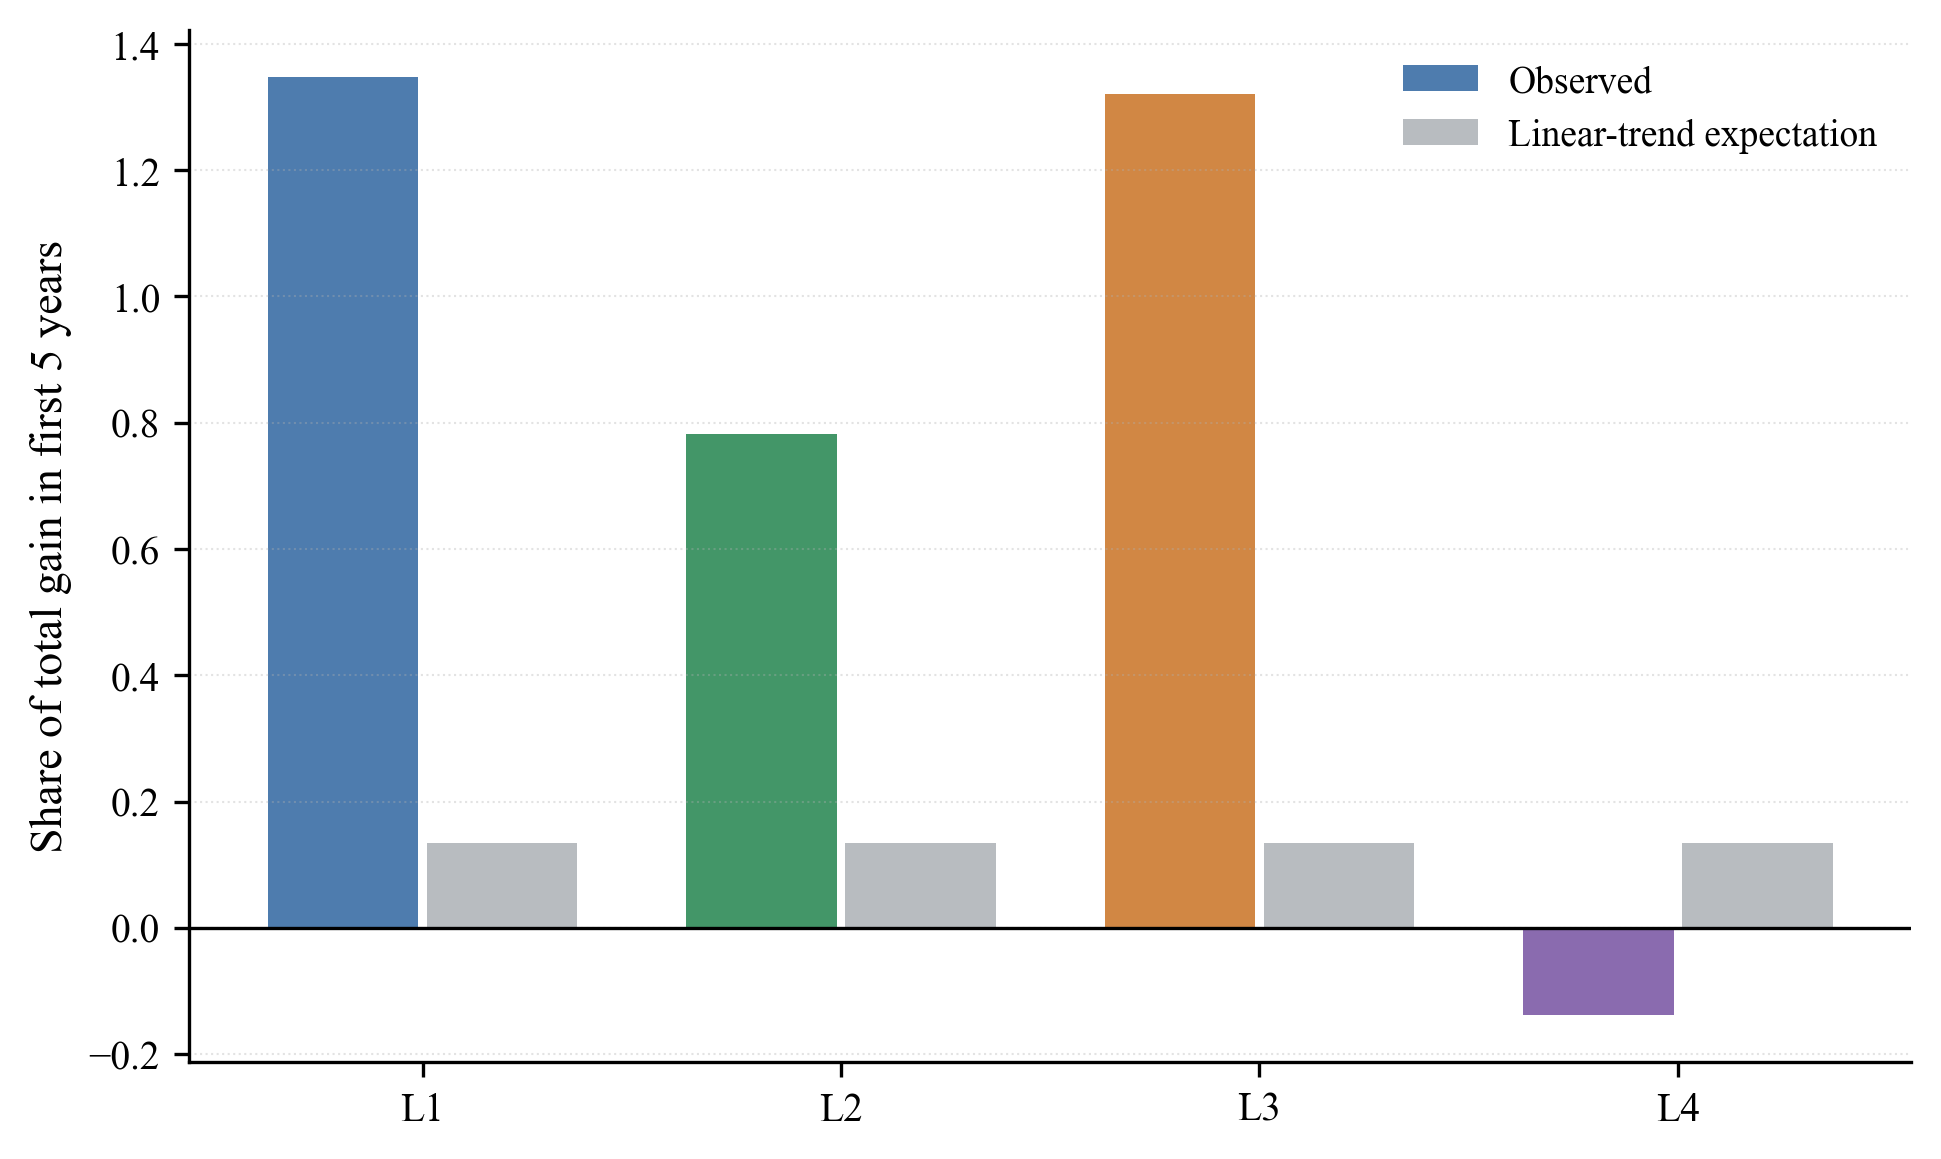
\includegraphics[width=0.75\textwidth]{figures/fig6_sharpness.png}
\caption{Sharpness of reform response. Blue bars: observed share of total post-1854 gain occurring within the first five years. Grey bars: the share expected under a uniform linear trend.}
\label{fig:sharp}
\end{figure}

Together, the SNR and sharpness results justify treating the Reform Acts as \emph{strategic discontinuities}: shocks that produce concentrated, punctuated reorganisation rather than gradual incremental change.

\subsection{Summary: strongest vs.\ suggestive findings}

Table~\ref{tab:strength} summarises the empirical evidence by strength of support. Two top-line claims --- that Reform Acts function as strategic discontinuities, and that higher-order dimensions respond disproportionately --- are robust across multiple complementary tests. The visual leapfrogging signature and the differential timing of reform response are strong but more descriptive. Several secondary claims (post-reform acceleration, capability-before-mission sequencing within the strategic axis) are directionally consistent but not statistically decisive on detrended series; these are preserved separately for follow-up work rather than carried in the core claim.

\begin{table}[t]
\centering
\caption{Strength of support, claim by claim}
\label{tab:strength}
\small
\begin{tabular}{p{6cm}lp{6cm}}
\toprule
Claim & Strength & Quantitative basis \\
\midrule
Reform Acts are sharp strategic discontinuities & STRONGEST & E1 SNR $\geq 1.5\times$ for L1, L3 at 1854; E2 sharpness $\sim 6$--$10\times$ linear-trend expectation \\
Higher-order dimensions respond disproportionately & STRONGEST & L4 norm.~1877 effect = $2.41\times$ pre-reform; L4 rel.~break = $3.63\times$ \\
Visual leapfrogging signature in normalised trajectories & STRONG & L4 grows multiple-fold above 1820--1853 baseline; L1, L2 stay near 1.0 \\
Differential timing of reform response across dimensions & STRONG & Event-time plots show L3 kink at 1854, L4 break at 1877; L1/L2 no visible kink \\
Post-reform acceleration concentrated in strategic dimensions & SUGGESTIVE & 1877--1900: L4 +266\%, L3 +113\%, L1 +8\%, L2 +4\% \\
Capability (L3) precedes mission (L4) within strategic axis & SUGGESTIVE & Pre-1750 rolling correlation L3-leads-L4 advantage 0.5--0.7; formal cross-lag tests on detrended series not significant \\
\bottomrule
\end{tabular}
\end{table}

% ===========================================================================
\section{Discussion}
\label{sec:discussion}
% ===========================================================================

\subsection{Mechanism}

We interpret the leapfrogging pattern as the product of three interacting forces. First, the Reform Acts imposed \emph{exogenous strategic mandates} --- expansion of teaching, abolition of religious tests, restructuring of the fellowship system --- that could not be met through marginal efficiency improvements. Second, the University's \emph{endowment-funded resource slack} (substantially augmented by rising 19th-century land rents) provided the financial capacity to invest in capability ahead of strategic clarity. Third, the absence of competitive pressure on Oxford's core mission meant that \emph{operational optimisation was not the binding constraint}; the binding constraint was external legitimacy. Together these conditions produced a textbook leapfrog: capability and mission moved first, while efficiency and process modernised at their own slower internal pace.

\subsection{Implications for contemporary AI transformation}

The mechanism we identify has direct contemporary relevance. Three implications stand out.
\begin{enumerate}
\item \textbf{Leapfrogging is likely common, not aberrant.} Firms investing in AI talent and organisational redesign ahead of operational optimisation are not failing to follow a sequential best practice; they may be responding rationally to external pressure (competitive, regulatory) that forces higher-order change first.
\item \textbf{Regulatory shocks function like the Reform Acts.} Emerging AI governance mandates plausibly play the role our Reform Acts play in this dataset: exogenous institutional triggers that force rapid capability build-up and mission redefinition ahead of process modernisation.
\item \textbf{Resource slack is a precondition for leapfrogging.} Well-resourced firms may dominate visible AI transformation not because they face uniquely strong AI pressure, but because they have the financial slack to invest in capability ahead of certainty about deployment. Fiscally constrained organisations cannot leapfrog; they must transform sequentially or not at all.
\end{enumerate}

\subsection{Boundary conditions}

We are explicit about what does and does not generalise from the Oxford case. The \emph{pace} of transformation (200 years) is pre-industrial and does not generalise to contemporary technology cycles. The \emph{institutional structure} (endowment-funded, monopoly position, no market competition for core mission) is unusual --- the closest contemporary analogue is well-capitalised firms with substantial retained earnings, not all firms. What does plausibly generalise is the \emph{mechanism}: that external institutional shocks can short-circuit operational-first sequencing and produce disproportionate higher-order transformation, conditional on adequate resource slack.

\subsection{What this report does not claim}

We are also explicit about what is \emph{not} supported by the data. We do not find robust evidence for a strict L1$\rightarrow$L2$\rightarrow$L3$\rightarrow$L4 sequential ordering; change-point ordering is partial and threshold-sensitive. We do not find statistically decisive evidence that capability expansion precedes mission transformation within the strategic axis once levels are appropriately detrended; the direction is consistent with the hypothesis, but formal cross-lag tests on first differences are not significant. We do not generalise our findings to AI transformation as a tested empirical claim; the AI analogy is mechanism-based, not evidence-based, and requires independent empirical validation in contemporary settings.

% ===========================================================================
\section{Conclusion}
\label{sec:conclusion}
% ===========================================================================

This report has used 200 years of Oxford University accounting data to document a sharp asymmetry in organisational transformation under institutional shocks. Higher-order dimensions of transformation --- capability expansion and mission redefinition --- responded disproportionately to the 1854 and 1877 Reform Acts, while lower-order dimensions --- efficiency and process modernisation --- barely registered the same events. The Reform Acts themselves behaved as strategic discontinuities: punctuated, concentrated reorganisations rather than triggers for gradual change. We interpret this pattern as evidence of organisational leapfrogging.

The mechanism --- exogenous institutional pressure short-circuiting the operational-first sequence --- is, we argue, a candidate explanation for the apparent ``out of order'' character of much contemporary AI transformation. We do not test that claim directly here. What we have done is provide a long-run, well-identified empirical case in which the leapfrogging pattern is unusually clean. Whether the same mechanism explains AI transformation today is an empirical question for a different paper.

% ===========================================================================
\section*{Data and code availability}
% ===========================================================================

\noindent The full ledger extraction pipeline, enriched annual panel, and analysis code are available in the project repository. Replication of the analyses in this report requires running \texttt{experiments/analysis/analysis\_v10.py} on the enriched data archive.

\appendix

\section{Supporting Figures}

Figures~\ref{fig:accel} and \ref{fig:event} provide additional descriptive support for the leapfrogging pattern. They are not load-bearing for the core empirical claim but help visualise the dynamics underlying Table~\ref{tab:its} and Table~\ref{tab:breaks}.

\begin{figure}[H]
\centering
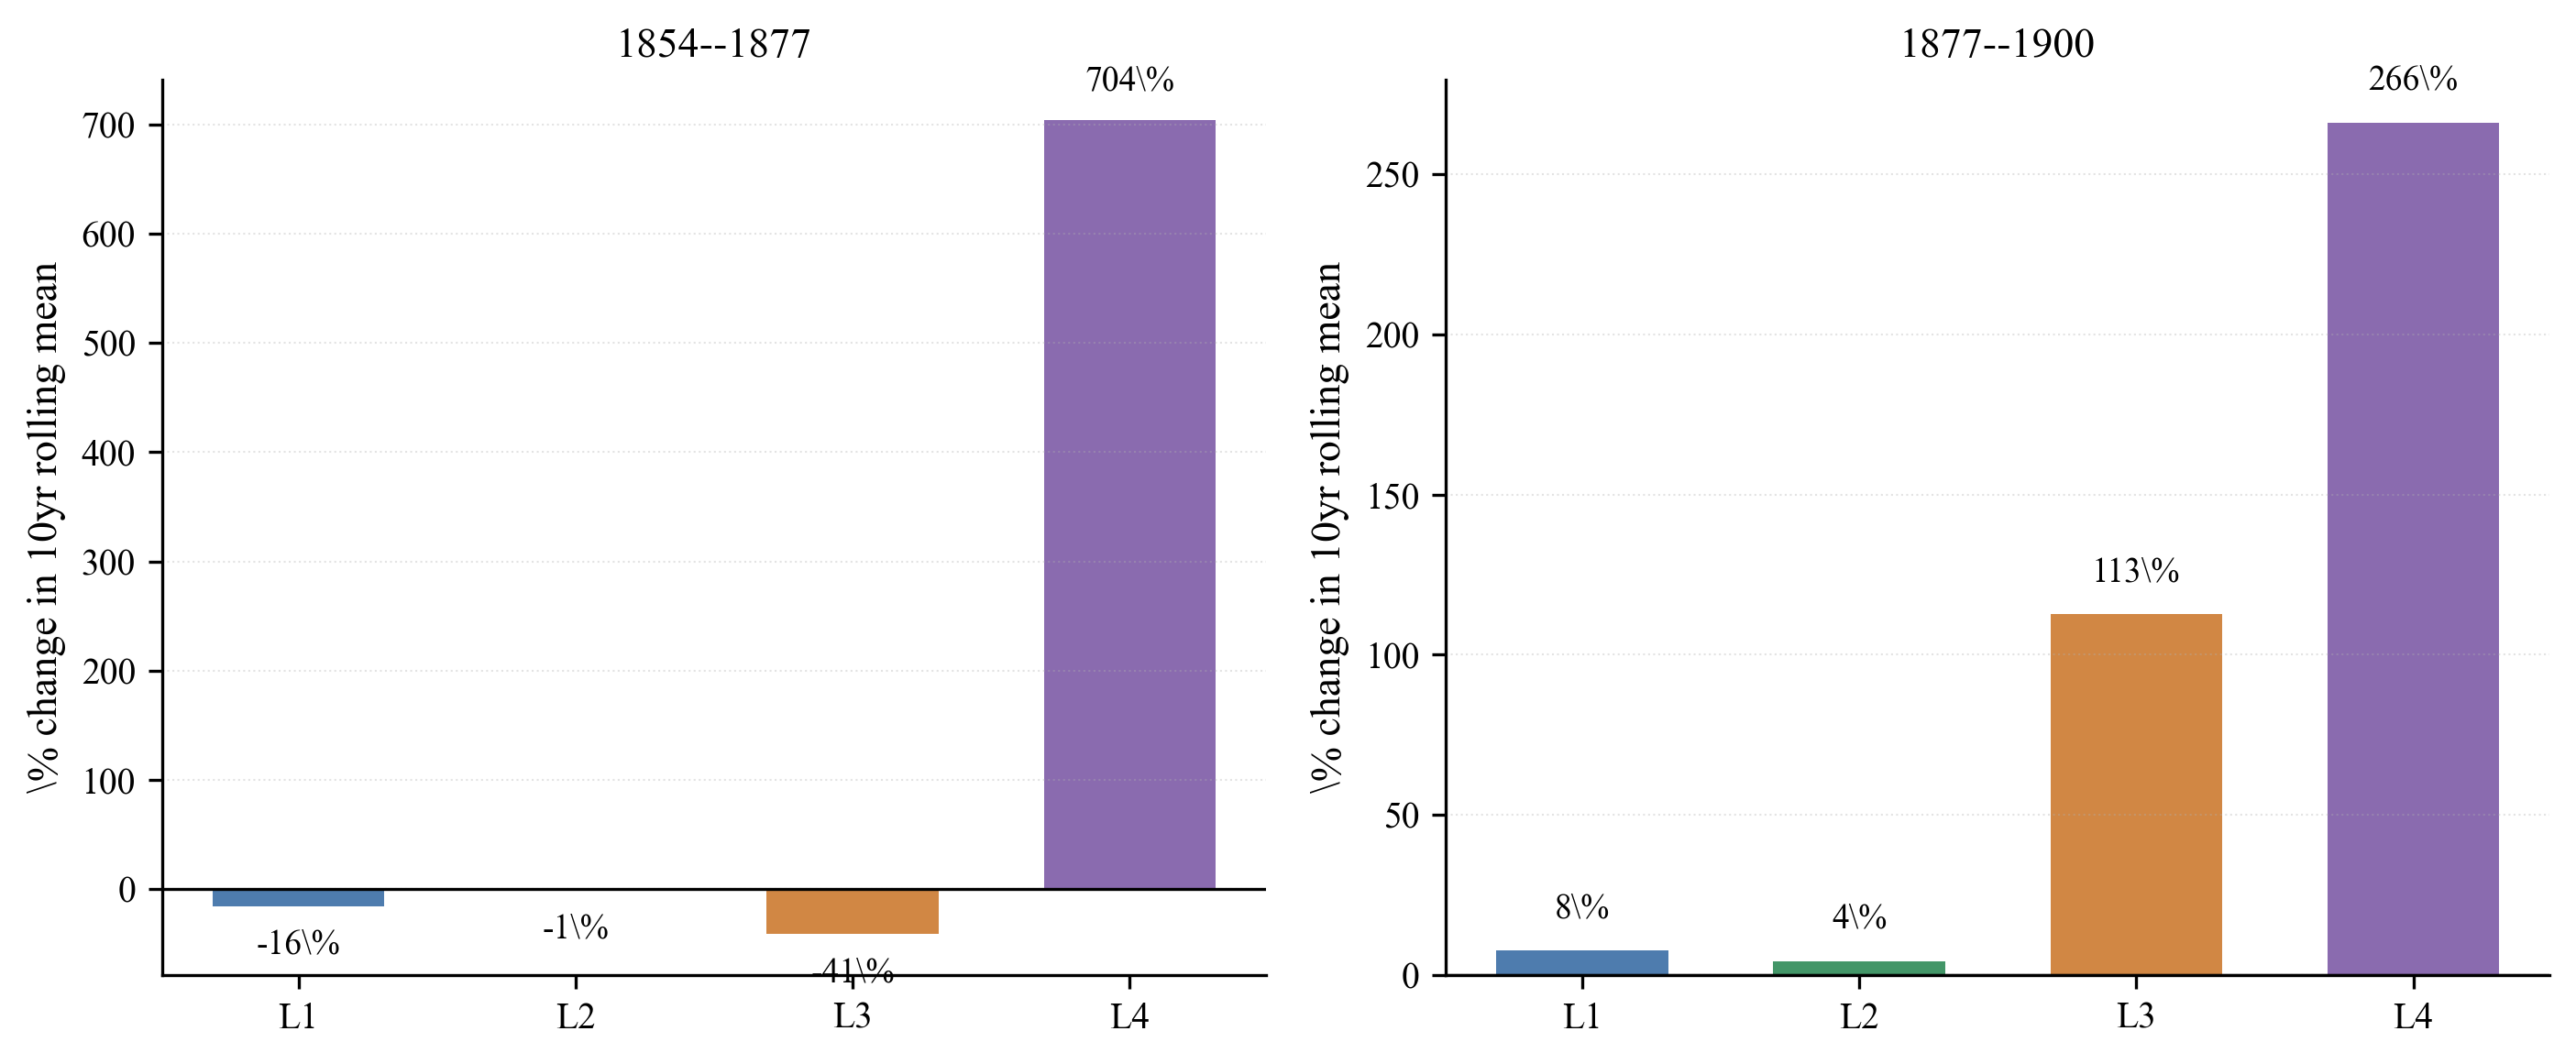
\includegraphics[width=\textwidth]{figures/figA1_acceleration.png}
\caption{Post-reform acceleration: \% change in 10-year rolling mean by dimension and window.}
\label{fig:accel}
\end{figure}

\begin{figure}[H]
\centering
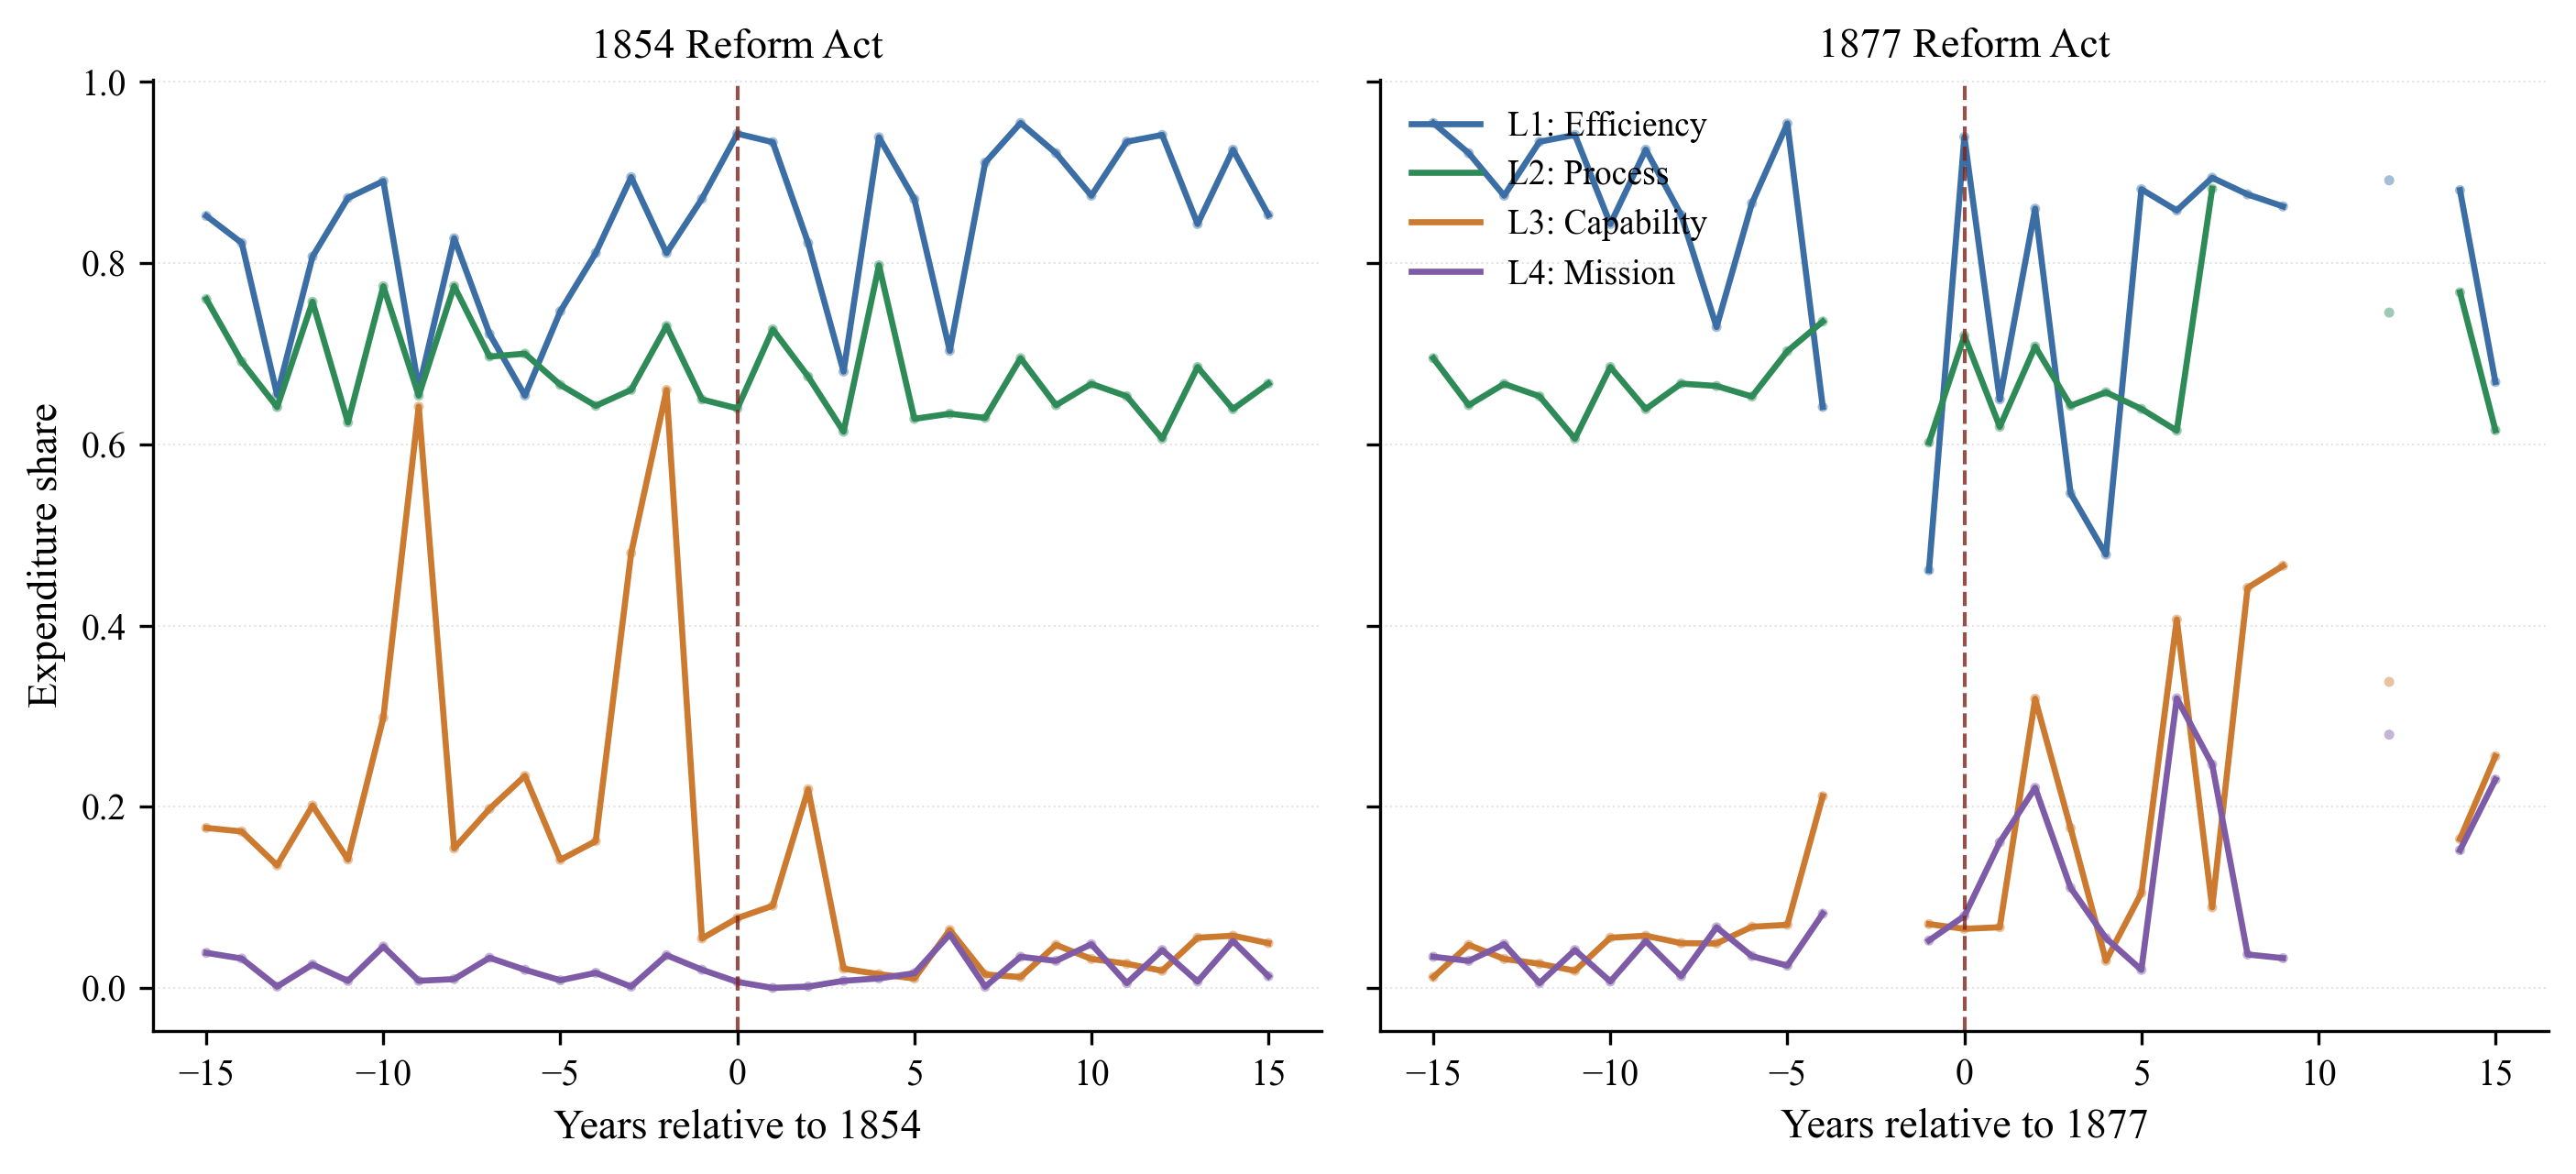
\includegraphics[width=\textwidth]{figures/figA2_eventtime.png}
\caption{Event-time response by dimension in a $\pm$15 year window around each Reform Act.}
\label{fig:event}
\end{figure}

\section{Research inventory: preserved findings for future papers}

Several empirically interesting patterns documented during the project are not central to the leapfrogging story and have been preserved separately as candidate future-paper directions. These include: (i) capability-before-mission sequencing within the strategic axis; (ii) tests of strict L1$\rightarrow$L2$\rightarrow$L3$\rightarrow$L4 ordering; (iii) Granger-causal chaining tests; (iv) the Latin-to-English semantic transition over the corpus; (v) income-source diversification dynamics; (vi) charity institutionalisation patterns; (vii) corporate-market transition in payment composition; (viii) payment modernisation in its own right; and (ix) the role of land-rent income as a resource-slack mechanism. A structured inventory of these findings, with empirical support, methodological approach, and source artifacts, is maintained as a companion document.

\end{document}
